\documentclass{article}


\usepackage{arxiv}

\usepackage[utf8]{inputenc} % allow utf-8 input
\usepackage[T1]{fontenc}    % use 8-bit T1 fonts
\usepackage{hyperref}       % hyperlinks
\usepackage{url}            % simple URL typesetting
\usepackage{booktabs}       % professional-quality tables
\usepackage{amsfonts}       % blackboard math symbols
\usepackage{nicefrac}       % compact symbols for 1/2, etc.
\usepackage{microtype}      % microtypography
\usepackage{lipsum}
\usepackage{float}
\usepackage{graphicx}
\usepackage{caption}
\usepackage{subcaption}
\usepackage{amsmath}

\usepackage{listings}
\usepackage{xcolor}	
\lstset { language=[ANSI]C++,
                backgroundcolor=\color{black!5}, % set backgroundcolor
                basicstyle=\ttfamily,
                keywordstyle=\color{blue}\ttfamily,
                stringstyle=\color{red}\ttfamily,
                commentstyle=\color{green}\ttfamily,
                morecomment=[l][\color{magenta}]{\#}
}

\title{GPU accelerated product of Chebyshev series}


\author{
  Kristoffer Lindvall\thanks{KTH profile: https://www.kth.se/profile/kfli} \\
  KTH Royal Institute of Technology, \\
  Division of Fusion Plasma Physics, \\
  Teknikringen 31, 114 28 Stockholm \\
  \texttt{kfli@kth.se} \\
  %% \AND
  %% Coauthor \\
  %% Affiliation \\
  %% Address \\
  %% \texttt{email} \\
  %% \And
  %% Coauthor \\
  %% Affiliation \\
  %% Address \\
  %% \texttt{email} \\
  %% \And
  %% Coauthor \\
  %% Affiliation \\
  %% Address \\
  %% \texttt{email} \\
}

\begin{document}
\maketitle

\begin{abstract}
The Generalized Weighted Residual Method (GWRM) is a numerical method used to solve partial differential equations. The solution is obtained by decomposing the entire spatial and temporal domain into a Chebyshev spectral space, where the Chebyshev coefficients are subsequently solved with a root solver. This allows for high-order solutions in both space and time without constraints such as the Courant-Friedrichs-Lewy (CFL) condition, perhaps even the parallelization of the temporal domain. The majority of the computation however is performed while computing the product of two Chebyshev series. The resultant Chebyshev coefficients $c_k$ is computed by performing several summations (of multiplications) in each element of $c$, this makes it a great candidate for GPU acceleration with Cuda. 
\end{abstract}


% keywords can be removed
\keywords{Chebyshev \and Spectral \and Cuda}


\section{Introduction}
Will it scale? That is one, if not the most, important questions that needs to be addressed when developing a new numerical method. Many advanced codes today harness the high performance computing power of cutting edge CPUs and GPUs. These new devices allow you to go from solving partial differential equations in a simple geometry with a couple dozen subdomains, to real-world CAD models of cars and airplanes with hundreds of thousands of subdomains. The problems become so large you even need advanced parallel techniques to store your solution!

Newly developed numerical methods such as the Generalized Weighted Residual Method, also called a Time-Spectral method, has quite a challenge when it comes to competition. Small-scale simulations have shown that the GWRM can compete with finite difference methods in both space and time, Runge-Kutta being prominent in the latter category. However, an evaluation on how the method will scale on modern hardware and with parallel techniques has yet to be done. 

In section 1 we will look briefly at the GWRM method and the individual components that can be treated with GPU acceleration. Section 2 will follow with a look at the Cuda toolkit that allows users to modify existing (C/C++) code with commands specific to GPUs. In Section 3 we will look at the results of our 1D and 2D Chebyshev product algorithm, followed by a discussion and conclusion.

\section{GWRM: A Time-Spectral Method}
The Time-Spectral method described here is a fully spectral method. A weighted residual method is used to decompose the real ordinary/partial differential equations into a set of algebraic equations where the Chebyshev coefficients are now the unknown. Here we will present the basic formulation of the Time-Spectral method followed by the specific formulas pertaining to the product of two Chebyshev series. 

\subsection{Basic formulation}
The basic formulation of the GWRM is presented here, although a thorough formulation of the Weighted Residual Method can be found in the article by J. Scheffel \cite{scheffel2012}. To continue, we wish to solve an arbitrary set of partial differential equations,
\begin{align}
\frac{\partial \vec{u}}{\partial t} = D[\vec{u}] + f,
\label{eq1}
\end{align}
where $u$ is the solution variable, $D$ is an arbitrary operator, and $f$ is forcing term. To highlight the difference between finite difference methods and spectral methods one needs to observe the type of approximation that is introduced in eq.~\ref{eq1}. Finite difference methods approximate the operators, typically the differential operator, in order to obtain an approximate solution of $u$ at a collection of points in space. Spectral methods, on the other hand, introduce an approximate ansatz of the solution variable $u$ itself. With Chebyshev polynomials this is seen as,
\begin{align}
u(t,x;p) \approx U(\tau,\xi;P) = \sum_{k=0}^{K}{}^{\prime}\sum_{l=0}^{L}{}^{\prime}\sum_{m=0}^{M}{}^{\prime} a_{klm}T_k(\tau)T_l(\xi)T_m(P)
\label{eq2}
\end{align}
where the prime symbol (${}^{\prime}$) denotes the first term in the respective series being multiplied by $1/2$. Here the Chebyshev coefficients are denoted by $a$, and the polynomials by $T$. Since the Cheyshev polynomials are orthogonal in the interval $[-1,1]$ so the variables space $x$, time $t$, and parameter $p$ need to be mapped from the real space to the chebyshev interval. This is done by the formula $\sigma=(z-\text{BMA}_z)/\text{BPA}_x$, where $\text{BMA}_z=(z_1+z_0)/2$ and $\text{BPA}_z=(z_1-z_0)/2$, and $z$ being the mapped variable. This gives us the new variables $\tau$, $\xi$, and $P$.

Next step is to introduce the solution ansatz eq. \ref{eq2} into the partial differential eq. \ref{eq1}. However, without any further consideration we can see that this will only increase the amount of unknowns in the system. The amount of unknowns need to be matched with the same amount of equations to make the system well-posed. To achieve this we use the weighted residual method which substitutes the ansatz into eq. \ref{eq2}, creates the residual of the system, and then integrates the residual, along with test functions and weights, over the entire domain. Here test functions are chosen as Chebyshev polynomials with their respective weight functions.
\begin{align}
\int_{p_0}^{p_1}\int_{x_0}^{x_1}\int_{t_0}^{t_1}RT_q(\tau)T_r(\xi)T_s(P)\text{w}_t\text{w}_x\text{w}p dtdxdp = 0.
\label{eq3}
\end{align}
Here the residual and takes the form,
\begin{align}
R = u(t,x;p) - \Big[u(t_0,x;p) + \int_{t_0}^{t_1}(D[u] + f)dt^{\prime}\Big]
\label{eq4}
\end{align}
With these in place the initial partial differential equations can be transformed into a set of algebraic equations,
\begin{align}
a_{qrs} = 2\delta_{q0}b_{rs} + A_{qrs} + F_{qrs}.
\label{eq5}
\end{align}
The $b_{rs}$ coefficients represent the initial conditions, $A_{qrs}$ are linear/nonlinear terms, and $F_{qrs}$ represent the forcing term. Boundary equations are substituted for the highest modes, depending on the order of the system. For example, a second order system requires that the two highest spatial modes be substituted for coefficients pertaining to specific boundary conditions.
\subsection{Chebyshev product}
The most computation intensive terms in the algebraic equations \ref{eq5} are the products between series of Chebyshev polynomials. We start by regarding the resultant Chebyshev series $h(t)$ of a Chebyshev series product, 
\begin{align}
h(t) \simeq \sum_{k=0}^K {}^{\prime}c_kT_k(\tau) = \sum_{i=0}^K {}^{\prime} a_iT_i(\tau) \cdot \sum_{j=0}^K {}^{\prime}b_jT_j(\tau).
\end{align}
Next, we introduce the formula for the product of two Chebyshev polynomials of the first kind,
\begin{align}
h(t) \simeq \sum_{k=0}^K {}^{\prime}c_kT_k(\tau) = \sum_{i=0}^K {}^{\prime}\sum_{j=0}^K {}^{\prime} \frac{a_ib_j}{2}[T_{i+j}(\tau)+T_{|j-i|}(\tau)].
\end{align}
Following the procedure laid out in the article by Riva et. al \cite{riva2017}, we wish to pair each index $k$ with all possible combinations of the indexes $i+j$ and $|j-i|$. This gives us the substitutions $j=k-i$, $j=k+i$, and $j=i-k$, so that,
\begin{align}
c_kT_k(\tau) = \sum_{i=0}^k {}^{\prime} \frac{a_ib_{k-i}}{2}T_k(\tau) + \sum_{i=1}^{K-k} {}^{\prime} \frac{a_ib_{i+k}}{2}T_k(\tau) + \sum_{j=1}^{K-k} {}^{\prime} \frac{a_{j+k}b_j}{2}T_k(\tau).
\end{align}
Eliminating $T_k(\tau)$ on both sides and substituting $j=i$ gives the final result,
\begin{equation}
c_k = \sum_{i=0}^k \frac{a_i b_{k-i}}{2} + \sum_{i=1}^{K-k}\frac{a_i b_{i+k}}{2} + \sum_{i=1}^{K-k}\frac{a_{i+k} b_i}{2}.
\label{1DCP}
\end{equation}
The first summation limit was chosen so that the upper limit will not become negative. The second and third summation limits were set so that no extra terms are computed that are not needed. If the resultant Chebyshev coefficients reach $K$, then the highest mode of the summation must also be $K$. Also, the second and third summation start at $i=1$ so that the $i=0$ term is only computed once.

The formula above can be used for an arbitrary amount of dimensions since the index procedure is the same.\footnote{Fabio Rivas' notes provided through private correspondence.} The formula for the product of 2D Chebyshev series is,
\begin{align}
c_{kl} = \frac{1}{4}&\sum_{i=0}^k \Bigg[\sum_{j=0}^l a_{i,j} b_{k-i,l-j} + \sum_{j=1}^{L-l} a_{i,j} b_{k-i,j+l} + \sum_{j=1}^{L-l} a_{i,j+l} b_{k-i,j}\Bigg] \\
&\sum_{i=1}^{K-k} \Bigg[\sum_{j=0}^l a_{i,j} b_{i+k,l-j} + \sum_{j=1}^{L-l} a_{i,j} b_{i+k,l+j} + \sum_{j=1}^{L-l} a_{i,j+l} b_{i+k,j} \Bigg] \nonumber \\
&\sum_{i=1}^{K-k} \Bigg[\sum_{j=0}^l a_{i+k,j} b_{i,l-j} + \sum_{j=1}^{L-l} a_{i+k,j} b_{i,j+l} + \sum_{j=1}^{L-l} a_{i+k,j+l} b_{i,j} \Bigg]. \nonumber
\label{2DCP}
\end{align}

\section{Cuda Toolkit}
The \verb+Cuda+ \verb+toolkit+ documentation can be found at (\url{https://docs.nvidia.com/cuda/}). The Cuda Toolkit is a parallel computing platform that allows users to adapt existing code (eg. Fortran and C/C++) to use GPUs. GPUs have been developed with massive multi-threading in order to handle large parallel computations. This allows GPUs to output a large amount of data to thousands of independent pixels on your screen without having to wait for the image to refresh. This is what GPUs were originally designed to do, however recent trends show just how wide spread the capabilities of GPUs really are. Now GPUs are routinely used in data analysis, computational fluid dynamics, neural networks and more.

The difference between a CPU and a GPU can be seen in Figure \ref{CPUvGPU}  (Accessed: 2019-09-12  \cite{CudaToolkit}). We see that the major difference being in the arithmetic operation and caching/control ratio, GPUs favoring arithmetic operations. This makes it possible to divide operations among the threads in parallel, with minimal data caching.
\begin{figure}[H]
\centering
  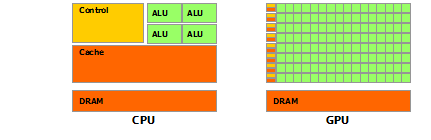
\includegraphics[width=\textwidth]{gpu-devotes-more-transistors-to-data-processing.png}
  \caption{Schematic of CPU and GPU architecture.}
  \label{CPUvGPU}
\end{figure}
The GPU hardware consists of \textit{Streaming Multiprocessors} (SM). These can be seen as self-contained units. The GPU can then achieve massive parallelism by fitting a host of SMs in one GPU. These SMs consist of Cuda cores, shared memory, a register file, load/store units etc. When data is sent to the GPU for calculation it is distributed to available SMs.

The Cuda programming model, on the other hand, provides a level of abstraction between software and hardware so that users can easily launch functions, called kernels, without necessarily having to know the exact GPU architecture. This means that we can choose to launch a kernel on $N$ number of threads, which then get distributed to the SMs. In order to optimize the kernels however, attention to the actual GPU architecture and memory sharing is absolutely essential. The two kernels written here will show the difference between a naive kernel, versus an optimized kernel. 

\subsection{Kernels}
The first kernel presented is a naive, or monolithic, kernel. The name monolithic refers to the thread strategy employed. For simplicity and clarification we will look at a Cuda code implementing the 1D Chebyshev product algorithm (eq. \ref{1DCP}). In each element $c_k$ we have a set of summations. The most straight-forward way to execute this on a GPU is to assign one thread per element $c_k$, i.e. monolithic. Thus each thread computes all of the summations/multiplications in that element. Below is a partial code showing the monolithic kernel. 
\begin{lstlisting}[caption={Monolithic kernel}]
int i = blockIdx.x * blockDim.x + threadIdx.x;
double sum;
if (i < n) {
   sum = 0.f;
   for (int j = 0; j<=i; j++){
      sum += a[j]*b[i-j];
   }
   for (int j = 1; j < n-i; j++){
      sum += a[j]*b[j+i] + a[j+i]*b[j];
   }
   c[i] = 0.5f*sum;
}
\end{lstlisting}
This kernel is a good first step in GPU acceleration. However, the drawbacks in this kernel is the choice of thread strategy. When implementing a thread strategy there are two main points that need to be addressed in order to optimize the kernel; Expose more parallel threads and efficiently use the memory. Thus we see where this kernel falls short. The monolithic kernel can be improved by launching multiple threads per vector element. One key algorithm that should be used when computing summations is the reduction sum algorithm. Also, we see that the first load from storage is $\text{a[j]}$, where all threads are trying to load the same value. For optimal memory coalescing we want adjacent threads to load adjacent values. Below is a partial code of the optimized kernel, called the Stride kernel.
\begin{lstlisting}[caption={Stride kernel}]
const unsigned row_mask = ~((0xFFFFFFFFU>>5)<<5);
int k = blockIdx.x;
int row_width = (((k)>(n-k))?(k):(n-k))+1;
int strides = (row_width>>5) + ((row_width&row_mask)?1:0);
int j = threadIdx.x;
double tmp_a;
double sum = 0.0f;
for (int s=0; s < strides; s++) {
  if (j < n) tmp_a = a[j];
  if (j <= k) sum += tmp_a*b[k-j];
  if ((j > 0) && (j < (n-k))) sum += tmp_a*b[j+k] + a[j+k]*b[j];
  j += 32;
}
for (int offset = warpSize>>1; offset > 0; offset >>= 1) {
  sum += __shfl_down_sync(0xFFFFFFFFU, sum, offset);}
if (!threadIdx.x) c[k] = sum*0.5f;
\end{lstlisting}
The thread strategy in the stride kernel is one block of threads per vector element. The stride occurs where threads in the block collect values in the summations, and then a reduction sum algorithm is performed. The threads in a warp (32 threads) can read the registers of all the threads in the warp (Cheng et. al \cite{Cheng2014}) so that they can quickly sum the collected values (see Figure~\ref{reducsum}). The reason why this is more efficient than writing to shared memory in a thread block is that the register is the fastest memory on a GPU. 
\begin{figure}[H]
\centering
  \includegraphics[width=.7\textwidth]{reduction.jpg}
  \caption{Schematic of the \underline{~}\underline{~}shuffle\underline{~}down\underline{~}sync() reduction sum.}
  \label{reducsum}
\end{figure}


\section{Results}
The simulations were computed on the Tegner system with a Tesla K80 GPU and an Intel(R) Xeon(R) CPU E5-2623 v3 @ 3.00GHz. The speedup results can be seen in Figure \ref{fig:fig1}. For the 1D case we have a nearly linear increase in speedup, and for the 2D case we see an exponential increase. The CPU code was run with openMP instructions and compiled with optimization flag -O3. For low numbers of Chebyshev modes in the 1D case ($N \simeq 200$) the CPU outperforms the monolithic kernel. The Stride kernel outperforms both the CPU and the monolithic kernel in all cases.
\begin{figure}[H]
  \centering
  \begin{subfigure}{.48\textwidth}
		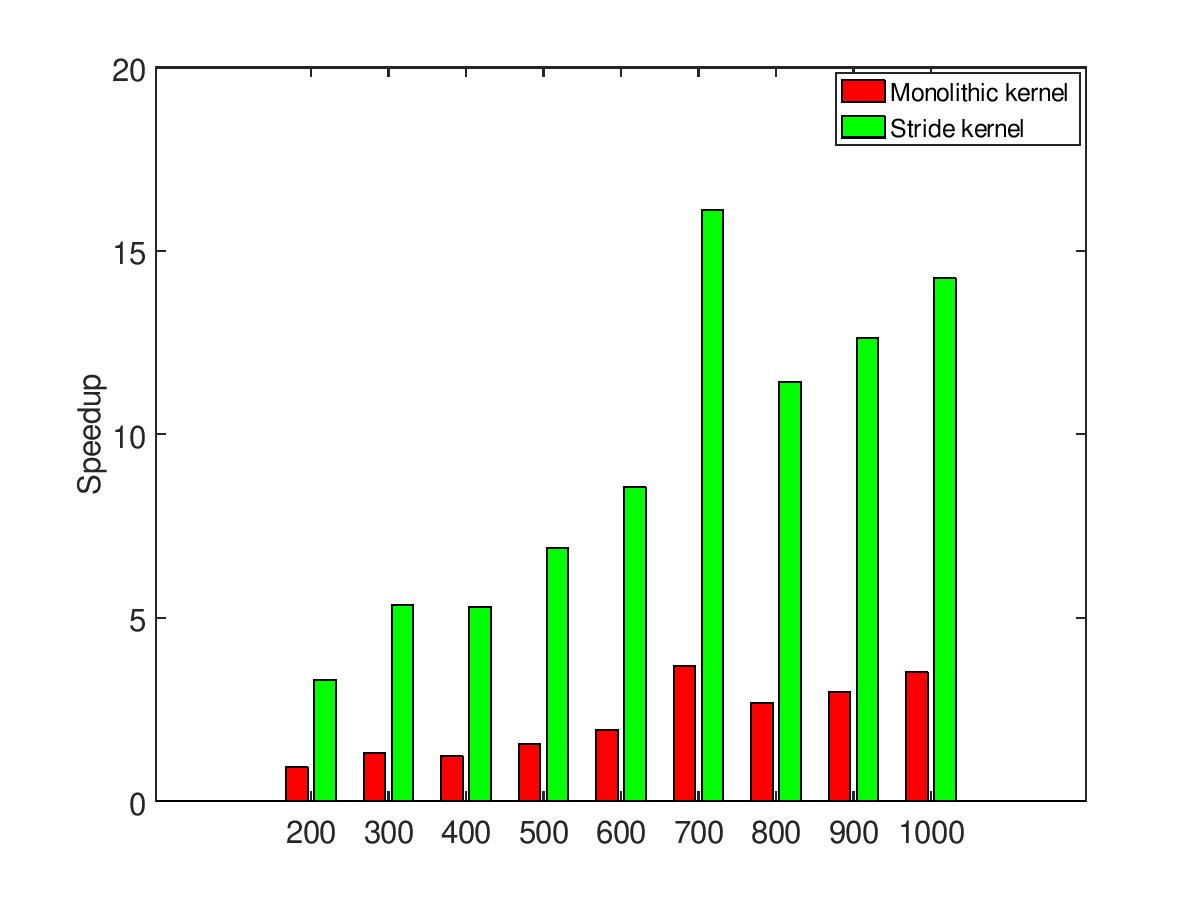
\includegraphics[width=\textwidth]{1Dparx.jpg}
		\caption{N Chebyshev modes.}
	\end{subfigure}
%%%%%%%%%%%%%%
	\begin{subfigure}{.48\textwidth}
		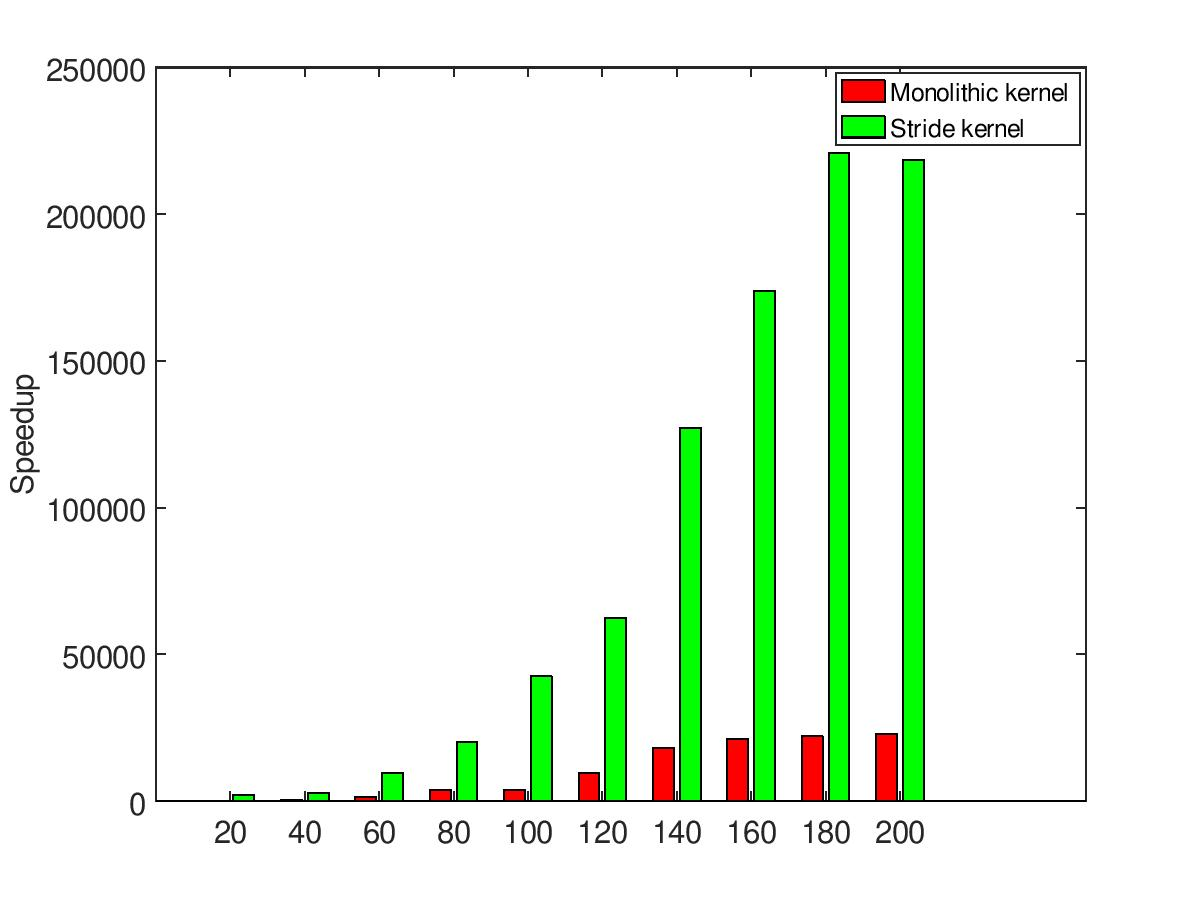
\includegraphics[width=\textwidth]{2Dpar.jpg}
		\caption{N=M Chebyshev modes.}
	\end{subfigure}
  \caption{GPU acceleration (Parallel CPU) of a 1D (a) and 2D (b) Chebyshev series product algorithm (Tesla K80). The two bars represent a naive monolithic kernel (\textit{red}) and an optimized striding kernel (\textit{green}).}
  \label{fig:fig1}
\end{figure}
The computation times for the 1D case ($N=200$ and $N=400$) can be seen in Table~\ref{tab:table1} and the 2D case ($N=M=100$ and $N=M=200$) can be seen in Table~\ref{tab:table2}. 
\begin{table}[h]
 \caption{1D Parallel CPU vs GPU kernels}
  \centering
  \begin{tabular}{lll}
    \toprule
    \cmidrule(r){1-2}
    Name     & Chebyshev modes (N)    & Time (ms) \\
    \midrule
    CPU   & 200   & 0.109  \\
    Mon.  & 200   & 0.118  \\
    Str.  & 200   & 0.033  \\
    \midrule
    CPU   & 400   & 0.196  \\
    Mon.  & 400   & 0.160  \\
    Str.  & 400   & 0.037  \\
    \bottomrule
  \end{tabular}
  \label{tab:table1}
\end{table}

\begin{table}[h]
 \caption{2D Parallel CPU vs GPU kernels}
  \centering
  \begin{tabular}{lll}
    \toprule
    \cmidrule(r){1-2}
    Name     & Chebyshev modes (N=M)    & Time (ms) \\
    \midrule
    CPU   & 100   & 170      \\
    Mon.  & 100   & 0.044    \\
    Str.  & 100   & 0.004    \\
    \midrule
    CPU   & 200   & 1093      \\
    Mon.  & 200   & 0.048     \\
    Str.  & 200   & 0.005     \\
    \bottomrule
  \end{tabular}
  \label{tab:table2}
\end{table}

\section{Discussion}
The optimized striding kernel manages to outperform both the CPU and the monolithic kernel. The main reason being the fact that the GPU is launching more threads, and these threads read data from the registers in their respective warp. The maximum speedup attained with the striding kernel is recorded for the 2D case $N=M=180$ at $S=220771$. This is a significant speedup result. 

The CPU function was programmed with openMP instructions. This applies threads, in this case 32, for the elements of vector $c$. The optimization flag -O3 was also used in order to optimize the instructions sent to the CPU. This was done in order to get a favorable CPU computation time. However, the CPU code could be improved with a better understanding of openMP instructions for parallelizing for loops. Some cases showed the serial CPU code performing similar to the parallel code. 

The computation times presented only include the time it takes for a kernel to execute. The copy function that sends data between CPU and GPU was not profiled due to the small array sizes. However, if larger arrays were to be transferred back and forth the transfer times should be included in the overall analysis. This should be taken in to account when applying the entire GWRM method on a GPU, since a lot of data will be transferred  between the host and device. Here it is worth mentioning that flattening 2D arrays to 1D arrays is beneficial, and has been included in the code here. Another form of overhead for the GPU is if 2D arrays need to be transposed for optimal memory coalescing. 

\section{Conclusion}
The GWRM relies heavily on the computation of algorithms such as the product of two Chebyshev series. This is a computation heavy algorithm that is not suited as a serial task. Therefore the Cuda toolkit was introduced to restructure the CPU host code so that the product could be performed on a GPU. 

The GPU acceleration achieved with a monolithic kernel is a good first step in parallelizing the Chebyshev product algorithm. However, to reach the full potential of the GPU a striding kernel was implemented that optimized several drawbacks of the monolithic kernel. First the thread strategy was changed to one thread block per output vector element, allowing for a reduction summation in each block. Second, the memory management was optimized by allowing threads in warps to read the registers of neighboring threads. This allows for efficient communication between the threads, leading to an optimal reduction sum. The most notable speedup results achieved with the GPU ranged roughly between $5k - 200k$ for the 2D case. The potential for parallel speedup is only increased when simulating in higher dimensions. 

Other algorithms such as the Chebyshev derivative and integral also show potential for being GPU accelerated. Already developed cuda algorithms such as the reduction sum and prefix scan are suitable for GWRM simulations. Future research on accelerating the GWRM method will focus on other algorithms such as the derivative and integral, efficient ways of finding roots to the algebraic equations, and optimizing the transfer of data between host and device.

\section*{Acknowledgment}
The author would like to acknowledge the help and guidance on striding kernels received from Stack Overflow user @Robert Crovella. His input was invaluable and a successful striding kernel is credited to him. Also a special acknowledgment of the staff and teachers at the PDC school for the lectures and lab sessions, and of course access to the PDC cluster.

\bibliographystyle{unsrt}  
%\bibliography{references}  %%% Remove comment to use the external .bib file (using bibtex).
%%% and comment out the ``thebibliography'' section.


%%% Comment out this section when you \bibliography{references} is enabled.
\begin{thebibliography}{1}

\bibitem{scheffel2012}
Jan Scheffel,
\newblock {\em A Spectral Method in Time for Initial-Value Problems},
\newblock {Amer. J. Comput. Math. 2, 2012}, 173--193.
\newblock {doi:10.4236/ajcm.2012.23023}

\bibitem{riva2017}
Fabio Riva, Lucio Milanese, and Paolo Ricci,
\newblock {\em  Uncertainty propagation by using spectral methods: A practical application to a two-dimensional turbulence fluid model},
\newblock {Phys. of Plasmas, 24, 2017}
\newblock {doi:10.1063/1.4996445}

\bibitem{CudaToolkit}
\newblock "The GPU Devotes More Transistors to Data Processing", Cuda Toolkit Documentation,
\newblock {[Online]. Available: https://docs.nvidia.com/cuda/cuda-c-programming-guide/index.html}

\bibitem{Cheng2014}
John Cheng, Max Grossman and Ty McKercher,
\newblock {\em Professional Cuda C Programming},
\newblock {Wrox Press, 2014}


\end{thebibliography}


\end{document}
